\chapter{路之尽头}

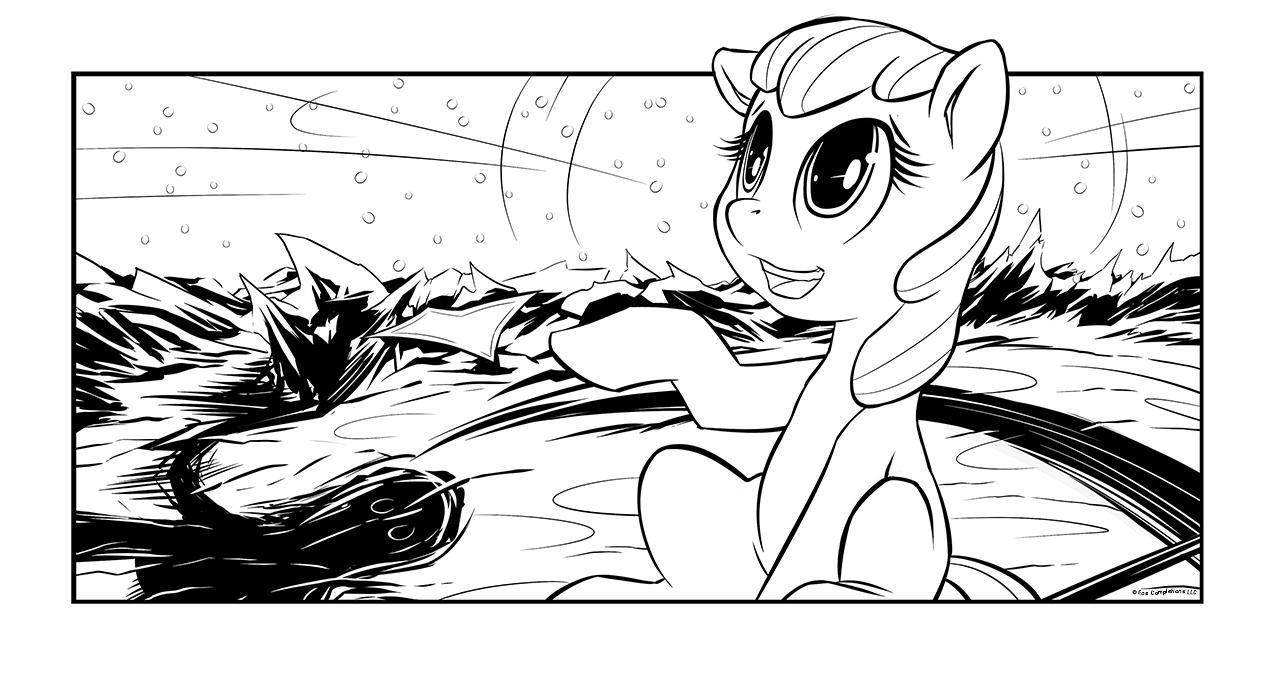
\includegraphics[width=0.9\linewidth]{image20.png}

\begin{intro}
    派对结束的时候,大家一起来个大拥抱吧!
\end{intro}

\daytimeplace{14}{12:35 AM}{翡翠海岸,52号国道南段}{Emerald Shores, Big 52 S Branch}

在拍打着海岸的阵阵波涛声中,帕比孤零零地面对着墓碑,而她的朋友在不远处争吵着。不过她唯一听到的就是在她脑中的低语,那个承诺给她美梦的低语。

「对,没错,请……让这一切都消失吧。」

赫瑞塔模模糊糊地听到帕比在她身后的低声念着,然后忽然感觉到一阵莫名的寒意,就好像刮起了一阵阴冷的夜风……她忽然觉得小雌驹刚才说的话有点不对劲。

大家全都回头看着快乐帕比,她在自言自语什么呢?消失?怎么消失?

赫瑞塔走过去,她可以看到帕比低着头闭着眼睛。小雌驹的鬃毛已经从之前的金色完全变成了夜空色。

「帕比?你还好吗?我……我觉得你鬃毛是不是有点……」

当帕比再一次开口说话的时候,却是另一个完全不同的声音,深沉而阴森,就好像在洞穴深处不断回荡的呼号。

「本宫终于亲临这个世界了,吾卑微的子民,还不赶紧对汝之新公主跪拜行礼!」

赫瑞塔歪着头挑起眉毛,「你丫说什么乱七八糟的,帕比?搞什么啊?」

小跟班的眼睛从红色变成了蓝色,慢慢走到帕比身后,像个卫兵一样笔挺地站着。那个黑化的帕比又说话了。

「本宫可不是快乐帕比,本宫乃星之子,怕音!汝等蝼蚁之辈的新公主,本宫将领导小马国崛起!」

诘责摇了摇头,看着融金问:「星啥?听起来像是某种上古斑马故事,星星什么的?」

老书记官的问题被赫瑞塔的暴笑打断了。

「怕音?你这个大反派的名字也太寒酸了吧,怕音是什么东东啊?你是自己想的么?」

羞得满脸通红的黑化帕比后退了一步,不过很快就恼羞成怒地大喝起来。「名字……名字什么的……收声,不准笑,愚民!这是汝等新公主之大名,还不快给本宫跪下!然后回到尔等故乡去宣布本宫临幸这个世界!」

快乐扳机嗤之以鼻,往前跨了一步,「不然呢?」

在怕音眼中的夜空色光芒一下子扩展到了小雌驹的全身。在她头上形成一个尖角,同时在背后展开了一对虚无的翅膀。

「不然,本宫会吞噬汝等灵魂!」

乐乐呆呆地看着那雌驹,而孤狼低声问诘责:「她能吃掉灵魂么?」

书记官看了看DJ,耸耸肩,「我怎么知道,如果她真是某种斑马黑魔法的产物……大概可以?不过我觉得她现在还没那么强。」

天马冷笑一声,「那就是不行啦?」

「并不全是,她还在显现阶段。你看她的翅膀和角还都只是虚影,而我想我知道怎么结束这场闹剧。」

在乐乐和那个生物对峙的时候,书记官低声和其他小马商讨着对策。

「我想我可以切断那个星灵和帕比的灵魂链接……如果怕音……呃……那东西没有灵魂以供给养,她就没办法在这个世界显现,自然就会被放逐回星界。」

「那么,你还等啥,邀请函么?」尸鬼问。

「不,我没办法自己施展这个魔法,这是一个又强大又复杂的法术,是一种超聚魔法,需要多个独角兽来施展……」

老赏金猎手说:「那么,你是想说,我们要被这个有这么孩子气名字的逗逼日翻了么?」

「喂,怎么,你们这些书呆子有什么好办法没有?」老白的脑袋挤进这仨小马围成的圈子中。

「技术上说,有,不过我需要几分钟搞定细节问题,帮快乐扳机让怕……这名字实在是……唉。」老书记官以蹄覆面,「好吧,反正让她忙着聊天,给我们争取点时间。」

老白点点头,然后走向另外仨马——赫瑞塔,坏枪和快乐扳机。

「我说,公主殿下,您刚才好像说了什么小马国崛起啥的?您可以详细说明一下如何做到么?别在没用的地方磨嘴皮了。」

梦魇暂时放下和赫瑞关于白痴名字问题的无营养争吵,转向新来的小马。「那易如反蹄,本宫的魔法比此等鼠辈强大万倍,本宫可以用法术治愈这腐朽的大陆,然后翻开小马国的新篇章!本宫决不允许吾之子民相互伤害,汝等粗鄙之辈的血腥争斗将被画上句号,汝等应该为本宫建造宏伟宫殿。汝只要为本宫送上贡品,而本宫将会解决汝等的一切问题!」

老白点了点头然后说:「好吧,听起来像那么回事……不过……你刚才说过贡品什么的是什么意思?」

那圣灵得意地坐下来,眼睛都乐得眯起来了,享受着被顶礼膜拜的快乐,「那是当然,本宫作为汝等的主宰。自然会要汝等做出一些……牺牲。嗯……每次满月的时候,每个城市献上一位小马做祭品就可以了,然后本宫会净化这片大地,保证汝等在本宫的统治下衣食无忧!」

乐乐皱起了眉头。「你……你要活祭做什么?」

怕音挥了挥蹄子,「和汝等无关。」

赫瑞和乐乐都惊得张大了嘴。雌驹正准备举起枪的时候,她注意到了老白的暗示又放下了。

这时候赫瑞说话了:「那么……你会把帕比还给我们么?」

梦魇有些惊讶的眨了眨眼睛,「什么,她才不会回来,在谁也不能伤害到她的地方,她正安享美梦,此乃吾等之约定!」

听到这句话,乐乐顿时大怒:「你说啥?帕比那么天真的孩子你都要骗,你的那些美梦全都是不存在的幻影!你……你居然欺骗一个孩子,骗她把美梦当成现实!放她回来!」

那怪物大笑起来:「汝等可笑至极!为何本宫会放弃如此甜美的灵魂美味,在她母亲陪伴的美梦之中,她将会长眠,从此彻底消失,这个残酷世界再也不会伤她分毫了。本宫绝不会再让那个孩子被你们所谓的现实所伤害。所以,那孩子将长眠不醒。另外,本宫特别开恩,提拔诸位成为本宫的信使,汝等现在就去小马国告诉子民本宫的驾临吧!」

「简而言之,」赫瑞抬着头,「你就是梦魇之月?」

「嗯,本宫尚未……好吧……正是……本宫是说……梦魇之月乃是比本宫更加古老而强大的前辈……」那个圣灵似乎陷入了沉思,不过马上又抬起头来,「不过本宫也足够让汝闭上那臭喙!」

赫瑞塔冷笑不已,「那么,简单的说,你丫还是个菜逼。嗯,梦魇菜逼。」

快乐扳机被这一句话逗得再也忍不住了,捂着肚子在地上笑得打滚,老白以蹄覆面,而其他三个小马回头看着这边,很好奇发生了什么。

「不准笑!本宫生气了!这个世界有这么多子民,本宫才不需要汝等……一……二……呃……反正很多个无用的笨蛋!」

赫瑞塔嗤之以鼻,「……你丫连四都数不到,就别装逼了好么?」

「汝……汝这个……蠢材!汝将付出代价!」

「不,她才不会!怪物!看招!」诘责站在了赫瑞塔面前,直视着梦魇的双眸,「以科学之名,我们会将你永远放逐!」

「哟呵?」那怪物咯咯笑着,虽然还气得满脸通红,但仍然不屑地挥了挥蹄子,「别逗本宫发笑了,科学?汝等是否明白本宫乃是何等存在?看在梦魇之月的份上,别说梦话了好么?」

诘责微微一笑,「你想听细节?好吧,仔细听好,我之前早就检查过帕比的防护服了,你能在这里显现的原因不过是因为某个呆瓜把死灵法术当生命维持法术用而已。不过我已经知道怎么纠正这个可怕的谬误了。虽然那魔法晶片几乎坚不可摧,但那里面的魔法却没那么稳定,这就是为啥你的翅膀和角还都只是虚无的火焰。不过现在这里有好几个独角兽,虽然他们不懂啥叫『魔法裂解术』,但我可以直接使用他们的魔力来施展这个超聚魔法。那么,现在猜猜看这个『魔法裂解术』要用在谁身上呢?」

「什……什么……?」那个梦魇大惊失色,后退几步。

「好了各位,我要准备法术了,你们只要放空脑子让我接管你们的力量,然后这场梦魇闹剧就此结束了!」

一道闪光从诘责的角尖上炸开,光芒跳跃到几个独角兽的角上,他们都一起将那个魔力聚集起来为超聚魔法添加魔力。

乐乐闭上眼睛,让魔力透过她的身体,然后坏枪和老白也一起做了,很快他们的角也一起发出同样炙热的光芒,照亮了整个山丘。

赫瑞塔被这强光逼得微微后退闭上眼睛,不过诘责刚才说的话让她很担心,他打算摧毁那个防护服上用作生命维持的死灵法术来毁灭那个梦魇,但那不是让帕比活着的东西么?

赫瑞塔转头对老书记官大叫着:「等等!你想杀了帕比么?」

诘责没有回答,但是被白光照亮的那个怪物惊恐的尖叫让赫瑞确认了自己的担忧。

「愚蠢之辈,如果你解除那个魔法,那孩子会和我一起死的!」

「不行,肏蛋!给老娘停下!你不能杀了帕比,天杀的独角兽!」赫瑞塔怒吼着冲向诘责,把他撞飞了出去,诘责仰面朝天地摔倒,失去了法术的专注。

那个白光射出的彩虹失去了焦点,飞得到处都是,就好像一个坏掉的迪斯科彩灯一样到处飞。

梦魇菜逼或者说怕音,小心地睁开眼睛,不知道发生了什么,不过看起来自己毫发无伤,看着面前几只满脸莫名其妙的小马,她的脸上露出了邪恶的微笑。

「哈……不管怎么说,帕比的狮鹫朋友最后还是有点用处的。下次挑战本宫之时,汝等还是别拉这种猪队友入伙了。」怪物大笑着:「噢,本宫说什么笑话呢,汝等已经没有下次了,因为汝等鼠辈现在就去死吧!」

诘责摇摇头站了起来,被赫瑞塔刚才那一撞搞的莫名其妙,「你……你为什么要打断魔法!你这个脑子里塞羽毛的蠢货!那法术就要完成了!」

另外几个独角兽也满脸恍惚,显然是被强力魔法的消耗搞得精疲力竭。融金正在推醒老白,赫瑞塔则冲向诘责,用爪子指着他叫着,「你……你不能把帕比从我身边带走!一定还有其它解决办法的,绝对会有的!」

「蠢货!那孩子已经死了!我们是在拯救52号国道!从你那快乐结局的美梦中醒来好么!」诘责怒斥着狮鹫,因为他们决胜的王牌被她给搞砸了,这样会害死很多小马。

梦魇享受着她对手的胜利美梦破灭的瞬间,「汝等的争吵何等有趣,本宫还真想再多欣赏一番,看鼠辈的丑恶内讧也是不错的消遣。不过现在本宫很忙,还有个王国要去统治。」怕音看了看双眸已经完全变成深空蓝色的跟班,那个中心城尸鬼已经变成了她忠心耿耿的侍卫,「游戏就此开始了。去吧,我的爪牙,教训这个臭嘴小鸡!」

跟班像猫扑老鼠一样扑向赫瑞塔,正在和诘责争吵的狮鹫完全没有注意到冲上来的尸鬼,甚至都没听到乐乐的警告。

尸鬼撞上狮鹫,扭作一团从山坡上滚了下去,赫瑞本能的反抗着,她的动物本能让她躲开了那小孩子强大的超自然力量,并且快速地反击着。他们化作一团蹄子和爪子的残影摔落到下面的海滩上。

看着她的爪牙和狮鹫滚出了视线,怕音叹了口气,「好吧,坏小鸡弄坏了我的玩具,看起来本宫还是自己动蹄……那么,谁想先死?」

孤狼和融金交换了一下视线,然后快速地跳起来把弹夹打空,子弹就像穿过黄油一样打穿了梦魇的身体。

帕比的胸口被打成了筛子,但是看起来完全没有用,因为下一瞬间那些洞都消失了。

「想要杀一个已经死掉的生物,是不是有点难度?」

怕音咯咯笑着用魔法抓起孤狼,然后把他扔向了一棵树。那天马重重撞在树桩上,随着一声黏黏糊糊的骨折声,倒在了地上,整个身体都向后弯折成了一个诡异的角度。

不过梦魇没有理会孤狼是不是死透了,转头面对着坏枪,「本宫看到汝还是拖家带口的来,何其可爱。汝等是想和那些老掉牙的戏剧一样『但求同年同月同日死么』?汝等有何遗言?」

「有,」老白举起包包里面的步话机,打断了怕音,「B计划,」他眯起了眼睛,「我们叫兄弟!」

远处传来一声炸雷,随之一发精确的狙击打穿了帕比的头盔,还轰掉了她的一条腿。

受伤的梦魇怒号着张开翅膀,飞上天空从云中招来闪电,雷霆如利剑般击中了远处的摩天轮,那个巨大的马造钢铁建筑在一阵烟尘之中轰然倒塌。

「不!灌木!」老白看着他侄子之前在的狙击位置已经成为一片废墟,这个……他完全没有想到会发生这种事情!

一排地对空导弹拖着长长的尾迹飞向天空中的梦魇,然后在她身边爆炸成无数火球,照亮了整个昏暗的天空。在他们的掩体之中,每一位铁骑卫都举起了他们的武器,向怪物的方向开始狂轰滥炸。

战斗开始了。

\horizonline

又黑,又冷,又湿,赫瑞塔呻吟着,她全身的骨头都在哀嚎,她完全不知道发生了什么,就记得有什么事情不对头。

在一阵粉色光芒中,有个甜甜的女声在低声耳语。

\emph{「亲,别担心,不过是你这个大坏蛋又干坏事了……没别的!」}

「坏啥?我死了?」狮鹫头疼得更厉害了,远处可以依稀听得到小马的尖叫声和爆炸声。但她可以清楚地感觉到,有什么东西,像是个粉色圆点,在她脑中跳跃着。

\emph{「笨笨小鸡,亲还没死呢。只不过是从六米高的高度大头朝下掉下来然后倒栽葱撞到烂石滩的后遗症而已啦。不过我可以肯定亲一点伤疤都不会有的!黛茜酱天天这么坠机也完全没有事!」}

「帕比?她怎么样了!我要救她!」

那个粉色圆点跳了跳,语气听起来就像是大姐姐在教训小孩子一样。\emph{「真的吗?但是看起来亲只是想要满足自己而已嘛!」}

「你……你他喵的叨叨什么鬼!我只想让她安全!」

\emph{「然后呢,让她永远永远都陪亲么?亲到底是想救谁,是可怜的小帕比,还是孤单的小赫瑞?」}

「老娘……我……我不知道……我只是想让她开心,让她露出笑容!她是如此特别,就像整个灰暗世界的一抹艳丽的色彩……我不想失去她,但是她除了自己妈妈什么都不想……就像……活在一个噩梦之中。」

\emph{「或许,她只是在做一个不知道如何醒来的美梦。或许,她需要她最最最要的朋友给她一点点点帮助。」}那个声音开始变化了,从一开始年轻雌驹的声音变成了一个老马的声音,但却又无比熟悉,让她想起来了太阳城那几天。\emph{「只剩下最后一步,找到帕比的「命运之石」,然后完成它的使命。」}

深吸一口气,赫瑞塔睁开了眼睛,发现自己正躺在乱石滩上。不远处是一个摔得粉身碎骨的太空士官长小跟班。那个生物似乎吸收了他们俩坠落的所有冲击力,现在就像一颗压扁的黄色橡皮糖一样贴在地上。赫瑞举起手枪,给那东西脑袋上补了两发,确保它完全死透彻了,然后检查周围。

在她头上,有一只小马被梦魇的夜空色魔法包围着,惨叫着飞出两百多米,然后啪叽一声栽进海里。

赫瑞没有理会那些上面那些战斗的喧嚣,给自己灌下一瓶治疗药水,开始找那块破石头。

「帕比的石头,帕比的石头!他妈的老娘怎么从这么多破石头中找一块石头?命运你妹的石头!」狮鹫恼怒地踢飞一块石头,那石头飞向一个生锈的铁盒子之后反弹的飞起来,在空中打着转,然后不偏不倚正中狮鹫双目之间。

「肏!」狮鹫一边揉着她的脑门一边捡起那块石头,她记得这块石头打中自己的声音,「这是你丫最后一次砸老娘的脑袋……然后……然后该干啥?你打中一个金属盒子,破石头,你想说啥?你是某种石头先知么?」赫瑞塔骂骂咧咧地走向那盒子,然后用「命运之石」砸向那盒子上的锁头。

「终于……」

咣!

「你丫……」

咣!

「还算……」

咣!

「有点用!」

咣当!

「很好,我们看看宝箱里面藏了什么?」

里面有几张纸片,一个老旧的阿杰玩偶,一些照片,赫瑞拿起照片看着他们。

其中之一是快乐帕比,不过稍微小一点,而且没有穿防护服,她正在插着四根蜡烛的大蛋糕面前开心地笑着,后面还有一些小马,看起来像是一个生日派对。

第二张照片是一个白色公马和紫色雌驹,他们站在一个老木牌面前,看起来他们是在苹果鲁萨门口,在两个小马之间坐着一个噘着嘴的快乐帕比,好像她不想拍照片或者完全不想去那里的样子。那个小雌驹看起来很年轻,或许只有三岁的样子……赫瑞塔转过照片,背面有一行字:「最后一次全家旅行。」

第三章照片是帕比穿着一件罩衫,带着一个蓝色的大大蝴蝶结,她正开心地笑着展示自己的新裙子,这一次在前面写着字,「帕比第一天去幼儿园」。

在最后一张照片的背面,年轻的佣兵发现后面写着这几行字。

\medskip

\wrpr{不管在哪里,不管是什么时候,在那遥远的彼端,我们会和爸爸再一次相聚。我以你为傲,妈咪永远会喜欢她的小小太阳。}

\wrpr{我爱你!}

\begin{flushright}
    \textbf{妈妈}
\end{flushright}

\medskip

一发导弹凌空爆炸,闪光照亮了赫瑞脸上流下的两行泪水。

佣兵叹了口气,终于抹去了模糊了双眼的泪,「她……她不属于这个地方……」赫瑞塔放下这些照片,「肏他娘,为什么要这样?为什么?!」

新的爆炸将天空染得火红,小马在那里和已经死去的东西战斗着,不断地死去,只是因为她自私地想要把幼驹留在自己身边。现在赫瑞知道自己该做什么了,虽然,这不意味着她真的想要这么做。

「不公平……这不公平……」

\horizonline

帕拉丁高斯瞪大眼睛,看着他发射的导弹在空中掉了个头,又朝自己飞了回来。

「高斯!」冷浴惊恐而无助地看着她最好的朋友在爆炸中消失,她愤怒而痛苦的视线转向梦魇,「臭婊子,为什么你不去死!」在她动力装甲两侧的转轮机炮疯狂地喷射着火舌,但是即使她打光了子弹,那个怪物也只是狂笑着把另一个新兵丢进大海。

怕音已经杀了两个铁骑卫,还把好几个小马丢进了大海,不过怎么才能一劳永逸地消灭这些家伙呢?这些笨蛋真的不知道什么叫决斗的规矩!她现在开始有点不耐烦了。虽然说杀掉小马很有趣,不过现在看起来这些家伙简直烦不胜烦,前仆后继根本杀不光的样子。而且她现在可有更重要的事情要做——比如说,统治世界之类的。

那么擒贼先擒王,这些蠢蛋的老大是谁呢?哦,对了,那个老书记官……怕音因为自己的小小邪恶脑瓜而坏笑着,「我说,穿披风的家伙在哪儿啊?」怕音落在老马的面前,张开她夜空色的翅膀邪笑着,「在这里啊,诘责,是吧?」就在那独角兽因为小雌驹心情突然变化而奇怪的时候,梦魇的笑容变得无比凶恶,「那么,去死吧!」怪物用魔法抓起老马的心脏,然后用力一捏,诘责闷哼一声倒了下去。

这个时候,赫瑞塔从悬崖边飞了上来,落在小山丘上的墓地边,面前的景象让她心中一紧。这都是她自私的错,小马在战斗,小马在死去,帕比绝对不会想要这样,该是结束这一切的时候了!

「帕比!帕比!听我说!」

不耐烦地叹了口气,梦魇转向狮鹫,「我说,还没轮到你呢?知道先来后到吗,等我先把这个杀掉之后再来杀掉你,别着急行不行?」

快乐扳机艰难地爬向诘责,卫兵雌驹绝望地想把老书记官救活过来。他们的抵抗就像纸片一样被小孩子扯得粉碎:融金正在那根穿透了他身体的树干上拼命挣扎着想要脱身,孤狼早因为脊椎骨折而昏了过去,即使是那些精锐的铁骑卫也被打得节节败退。难道这就是世界末日了么?他们都要死在这里了么?那一瞬间,乐乐觉得很伤心,她本来也想要个自己的孩子,这不公平……{}

「帕比,醒醒!你……你可以去见你妈妈的,真的!」赫瑞塔用她最高的声音尖叫着,她的嗓门确实很烦,「这臭不要脸的梦魇在骗你,你比她厉害多了!你是最棒的!」

黑化帕比哼了一声:「等不及去死了么?」夜空色魔法光芒笼罩在一块大石头上,然后径直朝狮鹫砸去,但是赫瑞灵巧地躲开了石块。「坏小鸡,别让本宫动怒好么。」

赫瑞塔直飞上天空,一个俯冲扑了上来,脑门紧紧地贴上了帕比的玻璃头盔,「帕比你这个笨蛋!你已经死了!死了!和你妈妈一样死翘翘了!难道你笨得连怎么死都不知道?别管这个蠢蛋,去找你的父母吧!」

「什么?」梦魇眨了眨眼睛,被狮鹫的突袭吓了一跳,她在说什么?她在和帕比说话?不……不不不不不……不可以!

「收声,她听不到你!」

「帕比,醒醒啊!你不用再留在这个世界了!我不需要你陪我!你应该离开了!我没关系……真的……」

一道夜空色的光芒笼罩了赫瑞塔的全身,让她身体在扭曲中发出断裂的脆响。怕音瞪着佣兵的双眸,她的声音充满了愤怒,充满了憎恶,「去!死!吧!」

赫瑞塔无法抵抗那强力的魔法,只是虚弱地笑着。

「帕比……你妈妈……就在那遥远的彼端……」

\horizonline

坐在一个池塘前,快乐帕比看着里面游泳的鱼儿,她周围的一切都如此宁静。皑皑白雪就像是星星从天上落下一般,覆盖了整个世界。她不觉得快乐,但是也不觉得悲伤,就像是在发呆一样,万事万物都模糊不清,也没什么意义。只有她,雪,还有水里的鱼儿。

帕比不记得自己在这里呆了多久,不过那不重要,她只是想忘记……忘记那些不想回忆的痛苦,或许真的有效,直到一条奇怪的金鱼从池塘里面探出头来。

「帕比你这个笨蛋!你已经死了!」

「虾米?」小雌驹歪着头,然后看了看自己的蹄子和尾巴,「我才没死,笨笨鱼!」

另一条鱼从池塘里面抬起头来,用女孩的声音说:「帕比,醒醒啊!你不用再留在这个世界了!」

「赫瑞?你怎么变成鱼了?」帕比咯咯笑着,「笨赫瑞,鱼不会说话的。」

寒霜开始冻结池塘的表面,但是第三条鱼从水中跳了出来,用赫瑞的声音说:「妈妈就在那遥远的彼端!」

\rcpr{「妈妈,爸爸去哪了?」}

\rcpr{「帕比,爸爸就在那彩虹的另一边……」}

\rcpr{「他……他会回来吗?」}

\rcpr{妈妈没有回答,但是帕比真的好想,好想,好想再见一次爸爸。}

\rcpr{「我……我们可以去找他么?」}

\rcpr{「没错,帕比……总有一天,不过不是明天,或者后天……在另外一个地方,在另外一个时间……我们最终会再一次团聚,好么?就是……就是在那遥远的彼端。」}

\rcpr{「萍琪毒誓?」}

\rcpr{「诚心发誓天上飞……」}

「眼里塞个蛋糕杯……」

帕比看着天空……终于看到了他。

「这次我是真的真的迟到了,虽然这个宇宙的所有时间都属于我,不过最近事情真的太多了,让我足足迟到两百多年!我可真不想来这里啊。」穿着黑色兜帽的骷髅马朝帕比走来。不过他看起来在自言自语,而不是在和帕比说话。

小雌驹笑了出来,那骷髅马真的好有趣,他就像那些坏脾气的退伍军马一样叨叨个不停。

「嗨,我是快乐帕比!你见过我妈妈么?」

「拜托!千万别祈祷!我要辞职了,或者退休了,或者先辞职再退休!」

骷髅马被小雌驹的咯咯笑声打断了。

「哇哦,骷髅马好有趣!」

停下了抱怨,那个灵魂收割者终于注意到了那个幼驹正在看着他,「你……你可以看到我?这是什么恶作剧么?如果这次又是恶作剧的话我真的要投降了……」

帕比歪着头。「恶作剧?绝对不是!上次我恶作剧我可是挨了好一顿打!」

那小马长舒一口气,然后坐了下来,「终于……」

帕比走到那个奇怪的公马身边,嗅着他的衣服,「呃……你是谁啊,漂漂骷髅马?」

「我?我是灵魂收割者,死神,终末,黑马……」看着那小雌驹一脸不解地眨着眼睛,骷髅发现自己只是在浪费好词,「不过那都是些无聊的名讳,我是那个引导小马走向他们来世的家伙。」

帕比一脸迷糊的表情问:「那么……你到底见过我妈妈没有?」

骷髅摇了摇头,「你还真是麻烦……」一张写着粉色字的银色机票轻轻飘落在帕比蹄子上,「小家伙,拿好这张银色机票,这可是给你的特快专机,感谢我吧!」

帕比睁大了眼睛,「我……我要去见妈妈了么?真的么?再也没有什么粉色箭头,或者坏机器,或者倒塌房子……只有……妈妈?」

死神点了点头,「没错,抱歉之前让你受苦了,让我以我自己的方式向你表达之前没有帮助你的歉意。」

帕比完全没有听到后半句,因为她已经开心的一蹦三尺高,「耶!」小雌驹紧紧抱了抱骷髅,然后回头看了一眼完全冻结的池塘。

「哦,对了,赫瑞!我要和我的朋友道别!」帕比转过头来,整个雪景顿时化作无数碎片,消失得无影无踪

她回到了那个墓地边的战场。

\horizonline

「……在那遥远的彼端……」狮鹫说完这句话之后,她双目失去焦点,昏了过去。

不过她刚刚说完这句话,那个梦魇的双眸就重新亮起了粉色的光芒,她的表情也完全变了,「拜拜赫瑞!一个漂漂骷髅马送我去妈妈在的地方了!还有一个超级闪闪的机票!」

最后一次,帕比眼中的粉色光芒消失了,她面前的HUD上亮起了红色的惊叹号。

「{\mt 警告,目标001快乐帕比无法定位,电池电量严重不足,警告,自动修理功能无响应,警告,硬件错误:未找到硬件。警告,即将关机,五……四……三……感谢您选择和平部,祝您有健康美好的一天,保重!}」

说完这些话之后,整个头盔上的HUD都消失了,只剩下怕音那张惊恐的脸瞪着空空如也的头盔。

那个怪物的魔力也消失了,被抓着的狮鹫落在不远处的山丘上,「汝等干了什么好事,蠢货!本宫要立刻杀了你们!汝等蝼蚁之辈!」展开它的翅膀,怪物想要放出一波新的魔法,但是她似乎有什么不对劲,因为那件防辐射服活像个破旧的皮球一样开始四处漏气,「怎么回事……本宫……我……我要融化了……不……不要!」粉色的气体从布料上的每一个破洞泄露出去,此刻,那个怪物身体只剩下一个完全的空壳。

「汝等!你们\ldots 你们别高兴得太早!本宫还会回来的!小马总会犯同样的错误,我要……啊啊!」梦魇的小脸化成了一滩粉色的粘液,把整个玻璃头盔溅成了粉色,一瞬间那个防辐射服似乎像个派对气球一样膨胀起来,然后在梦魇声调越来越高的尖叫中发出漏气的声音,像个被扎破的气球一样瘪了下去。

所有还能站起来的小马急忙抓起其他伤员,快速远离那团粉色的毒云。

「快走!赶紧躲开那东西!」冷浴抓起高斯的遗体紧跟着其他马。

在怕音的尖叫声中,小马四散而逃。

被半拖半拽的赫瑞塔期初还有点迷糊,所有东西觉得都非常遥远,她觉得自己好像在看不到的波涛之中上下起伏,在那恍惚的时候,佣兵好像听到了帕比的声音。

「喂……喂喂赫瑞!」

狮鹫呻吟着,那小鬼头从来不知道狮鹫的起床气有多大,如果她总是这样的话……{}

帕比显然不管赫瑞塔心中的抱怨,「听我说!我没什么时间了,但是我真的真的真的对不起,我真的要走了……我……我们还是朋友,对吧?」

还是朋友?真是个奇怪的问题,那小雌驹已经不只是一个朋友了,她是赫瑞塔生命之中更加重要的东西……

「真的?你这么喜欢我?我就知道!我们可以做姐妹!赫瑞塔·黛丝!我超级超级喜欢这个名字!」

狮鹫笑了起来,虽然还是被梦魇的魔法弄得迷迷糊糊。不过,赫瑞塔黛丝……真的……真的会这样么,被一个小马家庭收养?

「好了姐姐要走了我爱你拜拜!」

说完这句话,帕比的声音再一次消失,狮鹫也又一次失去了意识。

\horizonline

\daytimeplace{14}{17:00 AM}{翡翠海岸,52号国道南段}{Emerald Shores, Big 52 S Branch}

「{\rt 52号国道的朋友们,大家一切安好!这一次真的安好!这里是DJ好货!你正在收听的是52电台的新闻时间!}」

一段悠扬的音乐播放了一段时间。

「{\rt 我刚刚收到今天早上来自铁砧镇和花椰菜的新闻!我可以很负责任的说,野牛帮被击败了!呀呼!我的小马们,你没有听错,正义的伙伴在铁砧镇把强盗打得屁股开花!}」

DJ就在频道里面毫不专业地欢呼雀跃起来。

「{\rt 好吧好吧,我们接下来说现场状况……铁砧镇完全是个惨剧,很多成年小马都在围城中战死了,不过还有一些幸存者,大多都是老马和幼驹,还有一小队铁砧镇避难厩的卫兵,到现在为止我还没有幸存者清单,不过我会很快弄出一个,所以请在之后的新闻中静候。}」

「{\rt 另外一个新闻,闪耀峡谷被巨大的爆炸摧毁了,似乎是来自英克雷的袭……}」

快乐扳机关掉了电台,回头看着山丘,那粉色的云雾已经被风吹散,但已经把那棵大树染上了一层糖粉色。就在那颗大树下面,有两块墓碑。

赫瑞最后看了一眼她爪子里的石头。「命运之石」,狮鹫叹了口气,把帕比那沉甸甸的武器在蹄子里掂量了一下,然后将它放在了阴雨墓碑旁边的小土丘上,那里已经放着一个小马玩具——一只骑着红色滑板车的幼驹,还有一束鲜花。

年轻的佣兵张开喙想要说些什么,但是她什么也没说出来。白先生从小镇上搬来一块生锈的52号国道路牌,公马轻轻拍了拍赫瑞的肩膀,然后在金属牌上刻上了名字。

\begin{center}
    \textbf{——快乐帕比·黛西——}
\end{center}

站在新坟堆面前,乐乐神色黯然,「就只有这些了么,只是一个名字?看起来如此……冷冰冰……」

白苹果的首领耸了耸肩,「这是我们做事的办法,墓碑又不是为了展示什么。」公马视线转向不远处的另外一个墓穴,灌木的墓碑孤零零地立在这里,面对着北方,面对着盐块城的方向。老白摇了摇头看着乐乐。「她的墓碑又不是今天唯一一个墓碑。」

快乐扳机点了点头,叹了口气转向诘责,老独角兽正伤心的看着蹄子之中的一块兵牌,听到她走过来,连忙把那东西收了起来。

「DJ和尸鬼怎么样了?」

诘责叹了口气,「融金没有问题,他只需要点辐射就好……孤狼就没那么……好吧,我们会给他植入一个马造脊柱,但是我们现在没有设备,不知道他能不能撑过手术。你的男朋友在陪着他,你应该去看看他们。」

雌驹低下了头,「我……我很抱歉你失去那么多……我应该带上通道镇的所有卫兵,而不只是我和老枪……」

老书记官微微笑着:「不是你的错,我们都知道我们会有一天面对死亡,他们早已经立下誓言,为荣誉献上自己的生命。虽然这些话不能让他们起死回生,但是至少能让他们死得有价值。」

在乐乐离开之后,诘责走到了冷浴身边,和她一起坐在高斯的墓碑面前,雌驹正在无声地哭泣。那两个小马并不只是战友,而且他们也不只失去一个帕拉丁。

「他是个好朋友……你知道的,虽然他平时像个混蛋一样……」冷浴努力强忍住自己的泪水。

书记官点点头,用一只蹄子搂住了雌驹的脖颈,「没错,他很关心其他小马,他也知道什么最重要。」他的视线看着那四个墓碑,两个帕拉丁,两个侍从,虽然铁骑卫欠帕比的不只是这些,但还是很难以接受。而且他也没有责备狮鹫做的事,就算那其实并不正确,「我们失去了很多好伙伴,侍从糖花和学徒卷轴都很年轻,我必须通知他们的家属。」

冷浴叹了口气,泪水划过她的脸颊,「诘责,请你……请你告诉我,这一切都是值得的……我……我失去了那么多朋友……失去了我的挚爱……告诉我……告诉我他们的生命都没有白白浪费!」

「我们只是芸芸众生,冷浴,我们只是做我们力所能及的事情,让这个地方一天比一天更好。在最新的报告中,52号国道新一代得到的可爱标记里面,有建筑,农业和艺术的小马数量正在慢慢增加……或许这个世界会变得更好,或许我们的孩子能看到一个更美丽的小马国,」老书记官看着帕比的墓碑,「或许,有一天,这里将会是帕比那样天真烂漫的孩子一起玩乐,一起交朋友的美好地方……」

赫瑞塔揉了揉眼睛,目光从帕比的坟墓转到远处波涛起伏的大海上。年轻的佣兵四处看了看,确保没有谁在盯着她之后,悄悄从包包里面拿出了丝尾,她紧紧地把那玩偶抱在怀中,低声对那粉色的布偶说:

「别担心妹妹,明天会更好。」

\clearpage


~\vfill

\begin{note}
    升级(Lv 20)

    不对,你已经死了,抱歉孩子,胜败乃兵家常事……

    新任务专长解锁:小雌驹的幸运——需求:Lv 8 幸运7以上。

    「我们被包围了,对吧?那些机器到处都是,对吧?我们大概还剩下五发子弹,对吧?然后忽然听到楼下传来一声爆炸,那些机器被大公主才知道的什么东西扔石头打成了碎片,真的,我不骗你!」

    当面对机器群或者尸鬼群的时候,你会发现他们之中已经死了很多,被一块石头砸死的!上吧帕比!
\end{note}



